\begin{frame}{농장 관리(1245)}

\footnotesize

\begin{block}{문제}
농부 민식이가 관리하는 농장은 $N \times M$ 격자로 이루어져 있다. 민식이는 농장을 관리하기 위해 산봉우리마다 경비원를 배치하려 한다. 이를 위해 농장에 산봉우리가 총 몇 개 있는지를 세는 것이 문제다.

산봉우리의 정의는 다음과 같다. 산봉우리는 같은 높이를 가지는 하나의 격자 혹은 인접한 격자들의 집합으로 이루어져 있다. 여기서 "인접하다"의 정의는 X좌표 차이와 Y좌표 차이가 모두 1 이하인 경우이다. 또한 산봉우리와 인접한 격자는 모두 산봉우리의 높이보다 작아야 한다.

문제는 격자 내에 산봉우리의 개수가 총 몇 개인지 구하는 것이다.
\end{block}

\begin{block}{입력}
첫째 줄에 정수 $N(1 < N \le 100)$, $M(1 < M \le 70)$이 주어진다. 둘째 줄부터 $N+1$번째 줄까지 각 줄마다 격자의 높이를 의미하는 $M$개의 정수가 입력된다. 격자의 높이는 500보다 작거나 같은 음이 아닌 정수이다.
\end{block}

\begin{block}{출력}
첫째 줄에 산봉우리의 개수를 출력한다.
\end{block}

\end{frame}

\begin{frame}{예제 격자}
\centering

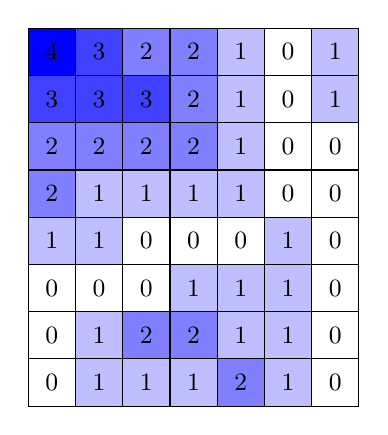
\begin{tikzpicture}[scale=0.6, every node/.style={font=\small}]

\foreach \x/\y/\v in {
1/1/4, 2/1/3, 3/1/2, 4/1/2, 5/1/1, 6/1/0, 7/1/1,
1/2/3, 2/2/3, 3/2/3, 4/2/2, 5/2/1, 6/2/0, 7/2/1,
1/3/2, 2/3/2, 3/3/2, 4/3/2, 5/3/1, 6/3/0, 7/3/0,
1/4/2, 2/4/1, 3/4/1, 4/4/1, 5/4/1, 6/4/0, 7/4/0,
1/5/1, 2/5/1, 3/5/0, 4/5/0, 5/5/0, 6/5/1, 7/5/0,
1/6/0, 2/6/0, 3/6/0, 4/6/1, 5/6/1, 6/6/1, 7/6/0,
1/7/0, 2/7/1, 3/7/2, 4/7/2, 5/7/1, 6/7/1, 7/7/0,
1/8/0, 2/8/1, 3/8/1, 4/8/1, 5/8/2, 6/8/1, 7/8/0
}{
    % 숫자 -> 색 변환 (0~4 → 0~100%)
    \pgfmathsetmacro{\percent}{25*\v}

    \fill[blue!\percent!white] (\x,-\y) rectangle ++(1,-1);
    \draw (\x,-\y) rectangle ++(1,-1);

    \node at (\x+0.5,-\y-0.5) {\v};
}

\end{tikzpicture}

\end{frame}

\setproblem{1245}

\begin{frame}[fragile, allowframebreaks]{김시온 소스 코드}
\inputminted{java}{\prob/Sion.java}
\end{frame}

\begin{frame}[fragile, allowframebreaks]{김준형 소스 코드}
\inputminted{java}{\prob/Junhyeong.java}
\end{frame}

\begin{frame}[fragile, allowframebreaks]{정의찬 소스 코드}
\inputminted{java}{\prob/Uichan.java}
\end{frame}

\begin{frame}[fragile, allowframebreaks]{서민종 소스 코드}
\inputminted{java}{\prob/Minjong.java}
\end{frame}

\begin{frame}[fragile, allowframebreaks]{손현준 소스 코드}
\inputminted{java}{\prob/Hyeonjun.java}
\end{frame}

\begin{frame}[fragile, allowframebreaks]{원찬혁 소스 코드}
\inputminted{java}{\prob/Chanhyeok.java}
\end{frame}

\begin{frame}[fragile, allowframebreaks]{김지훈 소스 코드}
\inputminted{java}{\prob/Jihoon.java}
\end{frame}

\begin{frame}[fragile, allowframebreaks]{임건애 소스 코드}
\inputminted{java}{\prob/Keonae.java}
\end{frame}
